\documentclass[hyperref={pdfpagelabels=true}]{beamer}
% By  using hyperref={pdfpagelabels=false} you get rid off:
% Package hyperref Warning: Option `pdfpagelabels' is turned off
% (hyperref)                because \thepage is undefined. 
% Hyperref stopped early 
%

\usepackage{lmodern}
% Using lmondern and you get rid off this:
% LaTeX Font Warning: Font shape `OT1/cmss/m/n' in size <4> not available
% (Font)              size <5> substituted on input line 22.
% LaTeX Font Warning: Size substitutions with differences
% (Font)              up to 1.0pt have occurred.
%

% If \title{…} \author{…} come after \begin{document} 
% you get the following warnig:
% Package hyperref Warning: Option `pdfauthor' has already been used,
% (hyperref) ... 
% So it is here before \begin{document}

% additional switch off the navigation symbols

\title{Bases de Dados Espaciais}   
\author{Joana Sim\~{o}es} 
\date{\today} 
 
\usepackage{beamerthemeshadow}

\newcommand{\soooo}{H$_2$SO$_4$}

\begin{document}
\setbeamertemplate{footline}[page number]
\setbeamertemplate{navigation symbols}{}
\begin{frame}
\titlepage
\end{frame} 

\begin{frame}
\frametitle{Table of contents}
\tableofcontents
\end{frame}
 

\section{Introducao} 
\begin{frame}
\frametitle{Apresentacao}
The Thermocouple String
\begin{itemize}
  \item Thermal expansions can occur very fast - 1s time resolution needed
  \item Thermal profile in the chamber can be inhomogeneous - multiple probes needed 
\end{itemize}
\begin{figure}
%\includegraphics[scale=0.3]{thermocoupleprobe.png} 
\end{figure}
\end{frame}


\begin{frame}
\frametitle{Motivacao para Este Talk/Workshop}
\begin{columns}
  \begin{column}{7cm}
  %\includegraphics<1> [scale=0.45,page=5]{../campaign/out/thermc_calib.pdf}
  %\includegraphics<2> [scale=0.45,page=4]{../campaign/out/thermc_calib.pdf}
  %\includegraphics<3> [scale=0.45,page=6]{../campaign/out/thermc_calib.pdf}
  \end{column}
  \begin{column}{5cm}
  \begin{itemize}
  \item<1-> PT100 probe is too slow to follow the experiment;
  \item<1-> We should get the radial structure of the temperature, is factory calibration right?
  \item<2-> Three point calibration...
  \item<2-> Noticeable difference from factory calibration;
  \item<3-> After calibration temperature spread decreases.
  \end{itemize}
  \end{column}
\end{columns}
\end{frame}

\begin{frame}
\frametitle{O que este Talk nao e...}
\begin{columns}
  \begin{column}{7cm}
  %\includegraphics<1> [scale=0.45,page=5]{../campaign/out/thermc_calib.pdf}
  %\includegraphics<2> [scale=0.45,page=4]{../campaign/out/thermc_calib.pdf}
  %\includegraphics<3> [scale=0.45,page=6]{../campaign/out/thermc_calib.pdf}
  \end{column}
  \begin{column}{5cm}
  \begin{itemize}
  \item<1-> PT100 probe is too slow to follow the experiment;
  \item<1-> We should get the radial structure of the temperature, is factory calibration right?
  \item<2-> Three point calibration...
  \item<2-> Noticeable difference from factory calibration;
  \item<3-> After calibration temperature spread decreases.
  \end{itemize}
  \end{column}
\end{columns}
\end{frame}


\section{Conceitos de Base de Dados}

\subsection{BD como Modelos de Realidade}

\begin{frame}
\frametitle{The UV System}
The UV Fibre and SABRE II\\
\begin{overprint}
\begin{figure}
\includegraphics[scale=0.2,page=5]{uv-harness_2378_500x500.jpg}
\end{figure}
\begin{figure}
\includegraphics[scale=0.3,page=5]{250px-Lightsaber_blue.png}
\includegraphics[scale=0.3,page=5]{250px-Lightsaber_blue.png}  
\end{figure}
\end{overprint}
\end{frame}


\begin{frame}
\frametitle{UV Fibre/UV Sabre II}
\begin{columns}
  \begin{column}{5cm}
  \begin{itemize}
  \item<1-> \textbf{UV Fibre}
  \item<1-> Stepping up the UV: $[$\soooo$]$ builds within t$\simeq$6 min;
  \item<1-> $[$\soooo$]$ changes almost one order of magnitude, UV from 0\% to 100\% ;
  \item<2-> \textbf{UV Sabre II}
  \item<2-> Similar to UV Fibre, but a bit weaker;
  \item<2-> UV fibre and UV Sabre II add together.
  \item<3-> $[$\soooo$]$ - same time to decay and to grow.
  \end{itemize}
  \end{column}
  \begin{column}{10cm}
  %\includegraphics<1>[scale=0.45,page=4]{../campaign/cigar_h2so4.pdf}
  %\includegraphics<2>[scale=0.45,page=7]{../campaign/cigar_h2so4.pdf} 
  %\includegraphics<3>[scale=0.45,page=6]{../campaign/cigar_h2so4.pdf} 
  \end{column}
\end{columns}
\end{frame}

\begin{frame}
\frametitle{UV Fibre/UV Sabre II}
\begin{columns}
  \begin{column}{5cm}
  \begin{itemize}
  \item Light intensity dependence on UV aperture is almost linear!
  \end{itemize}
  \end{column}
  \begin{column}{10cm}
  %\includegraphics[scale=0.45,page=5]{../campaign/cigar_h2so4.pdf} 
  \end{column}
\end{columns}
\end{frame}



\subsection{BD e SIG}
\frametitle{The CIGAR}
\begin{frame}
The CIGAR\\
\textbf{C}orona \textbf{I}on \textbf{G}enerator for \textbf{A}erosol \textbf{R}esearch
\begin{figure}
%\includegraphics[scale=0.3,page=5]{Guantanamera-cigar-2.jpg} 
\end{figure}
\end{frame}

\begin{frame}
\frametitle{CIGAR (+)}
\begin{columns}
  \begin{column}{5cm}
  \begin{itemize}
  \item<1> Single polarity ions;
  \item<1> The small ion concentration has a limited lifetime;
  \item<1> Big ions have a really long lifetime;
  \item<1> No ion recombination!
  \end{itemize}
  \end{column}
  \begin{column}{10cm}
  %\includegraphics<1>[scale=0.45]{../campaign/cigar.pdf}
  \end{column}
\end{columns}
\end{frame}

\begin{frame}
\frametitle{CIGAR +/-}
\begin{columns}
  \begin{column}{5cm}
  \begin{itemize}
  \item<1-> \textbf{CIGAR -}
  \item<1-> Stepping up the UV: $[$\soooo$]$ builds within t$\simeq$3 min;
  \item<1-> $[$\soooo$]$ changes 4x;
  \item<2-> \textbf{CIGAR +}
  \item<2-> Same growing time
  \item<2-> $[$\soooo$]$ changes 10x;
  \item<3-> $[$\soooo$]$ - Decay time t$\simeq$4 min.;
  \end{itemize}
  \end{column}
  \begin{column}{10cm}
  %\includegraphics<1-2>[scale=0.45,page=2]{../campaign/cigar_h2so4.pdf}
  %\includegraphics<3>[scale=0.45,page=3]{../campaign/cigar_h2so4.pdf}
  \end{column}
\end{columns}
\end{frame}

\subsection{Summary}
\begin{frame}
\frametitle{Sulphuric Acid Production}
\begin{columns}
  \begin{column}{5cm}
  \begin{itemize}
  \item<1> $[$\soooo$]$ has a linear dependence on UV\%
  \item<1> CIGAR (+) Produces more $[$\soooo$]$ than the UV System;
  \item<1> UV Sabre II is weaker than UV Fibre;
  \item<1> UV Sabre II can produce well mixed \soooo;
  \item<1> Both CIGARs can be used to produce a huge amount of ions (no recombination);
  \end{itemize}
  \end{column}
  \begin{column}{10cm}
  %\includegraphics<1>[scale=0.45,page=10]{../campaign/cigar_h2so4.pdf}
  \end{column}
\end{columns}
\end{frame}


\section{SGBD com Extensoes Espaciais} 
\subsection{Software Livre e de Codigo Aberto (FOSS)}
\begin{frame}
\frametitle{[H2SO4] Depletion/Evaporation}
\includegraphics<1>[scale=0.35,page=1]{runs_for_talk.pdf}
\includegraphics<2>[scale=0.35,page=3]{runs_for_talk.pdf}
\includegraphics<3>[scale=0.35,page=2]{runs_for_talk.pdf} 
\end{frame}


\begin{frame}
\frametitle{[H2SO4] Depletion/Evaporation}
[H2SO4] Depletion/Evaporation
\begin{itemize}
  \item It appears that sulphuric acid comes from droplets when they evaporate!
\end{itemize}
\end{frame}


\end{document}

\begin{frame}
\frametitle{lists with single pause}
\begin{itemize}
\item keyword  \pause 
\item still another keyword
\end{itemize} 

\end{frame}

\begin{frame}
\frametitle{lists with pause}
\begin{itemize}[<+->]
\item keyword  
\item still another keyword
\item a third one 
\end{itemize} 
\end{frame}


\subsection{Lists II}
\begin{frame}
\frametitle{numbered lists}
\begin{enumerate}
\item keyword
\item still another keyword
\end{enumerate}
\end{frame}

\begin{frame}
\frametitle{numbered lists with single pause}
\begin{enumerate}
\item keyword  \pause 
\item still another keyword
\end{enumerate}
\end{frame}

\begin{frame}
\frametitle{numbered lists with pause}
\begin{itemize}[<+->]
\item keyword  
\item still another keyword
\item a third one 
\end{itemize} 
\end{frame}


\section{Section no.3} 
\subsection{Tables}
\begin{frame}
\frametitle{Tables}
\begin{tabular}{|l|c|r|p{1.5 cm }|}
\hline
left & centers & right & width \\
l & C & r & p \\
\hline
\end{tabular}
\end{frame}


\begin{frame}
\frametitle{Tables with pause}
\begin{tabular}{c c c}
A & B & C \\ 
\pause 
1 & 2 & 3 \\  
\pause 
A & B & C \\ 
\end{tabular} 
\end{frame}


\section{Section no. 4}
\subsection{blocs}
\begin{frame}
\frametitle{blocs}

\begin{block}{title of the bloc}
bloc text
\end{block}

\begin{exampleblock}{title of the bloc}
bloc text
\end{exampleblock}


\begin{alertblock}{title of the bloc}
bloc text
\end{alertblock}
\end{frame}


\section{Section no. 5}
\subsection{split screen}

\begin{frame}
\frametitle{splitting screen}
\begin{columns}
\begin{column}{5cm}
\begin{itemize}
\item Beamer 
\item Beamer Class 
\item Beamer Class Latex 
\end{itemize}
\end{column}
\begin{column}{5cm}
\begin{tabular}{|c|c|}
\hline
\textbf{Instructor} & \textbf{Title} \\
\hline
Sascha Frank &  \LaTeX \ Course 1 \\
\hline
Sascha Frank &  Course serial  \\
\hline
\end{tabular}
\end{column}
\end{columns}
\end{frame}

\subsection{Pictures} 
\begin{frame}
\frametitle{pictures in latex beamer class}
\begin{figure}
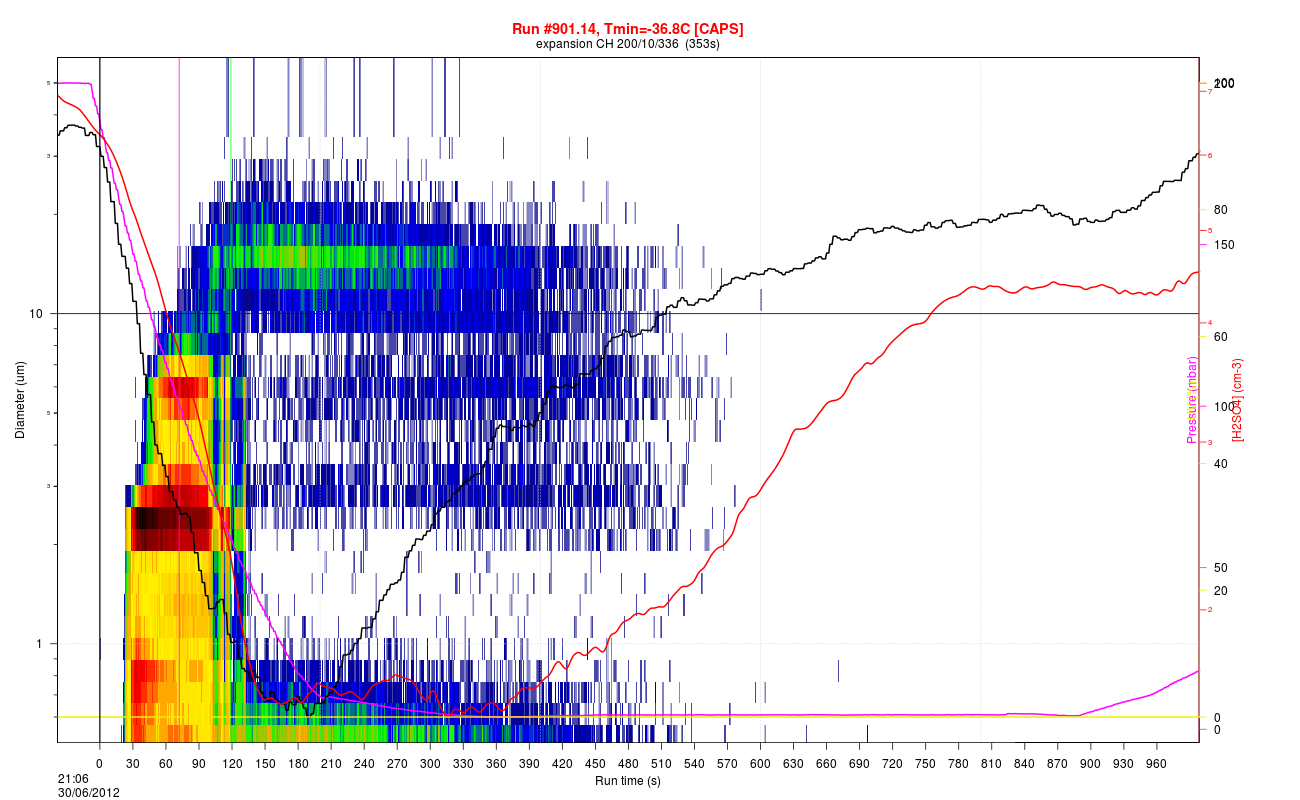
\includegraphics[scale=0.4]{runs_for_talk01.png} 
\caption{show an example picture}
\end{figure}
\end{frame}

\subsection{joining picture and lists} 

\begin{frame}
\frametitle{pictures and lists in beamer class}
\begin{columns}
\begin{column}{5cm}
\begin{itemize}
\item<1-> subject 1
\item<2-> subject 2
\item<3-> subject 3
\end{itemize}
\vspace{3cm} 
\end{column}
\begin{column}{5cm}
\begin{overprint}
\includegraphics<1>[scale=0.1]{runs_for_talk01.png}
\includegraphics<2>[scale=0.1]{runs_for_talk02.png}
\includegraphics<3>[scale=0.1]{runs_for_talk03.png}
\end{overprint}
\end{column}
\end{columns}
\end{frame}

\subsection{pictures which need more space} 
\begin{frame}[plain]
\frametitle{plain, or a way to get more space}
\begin{figure}
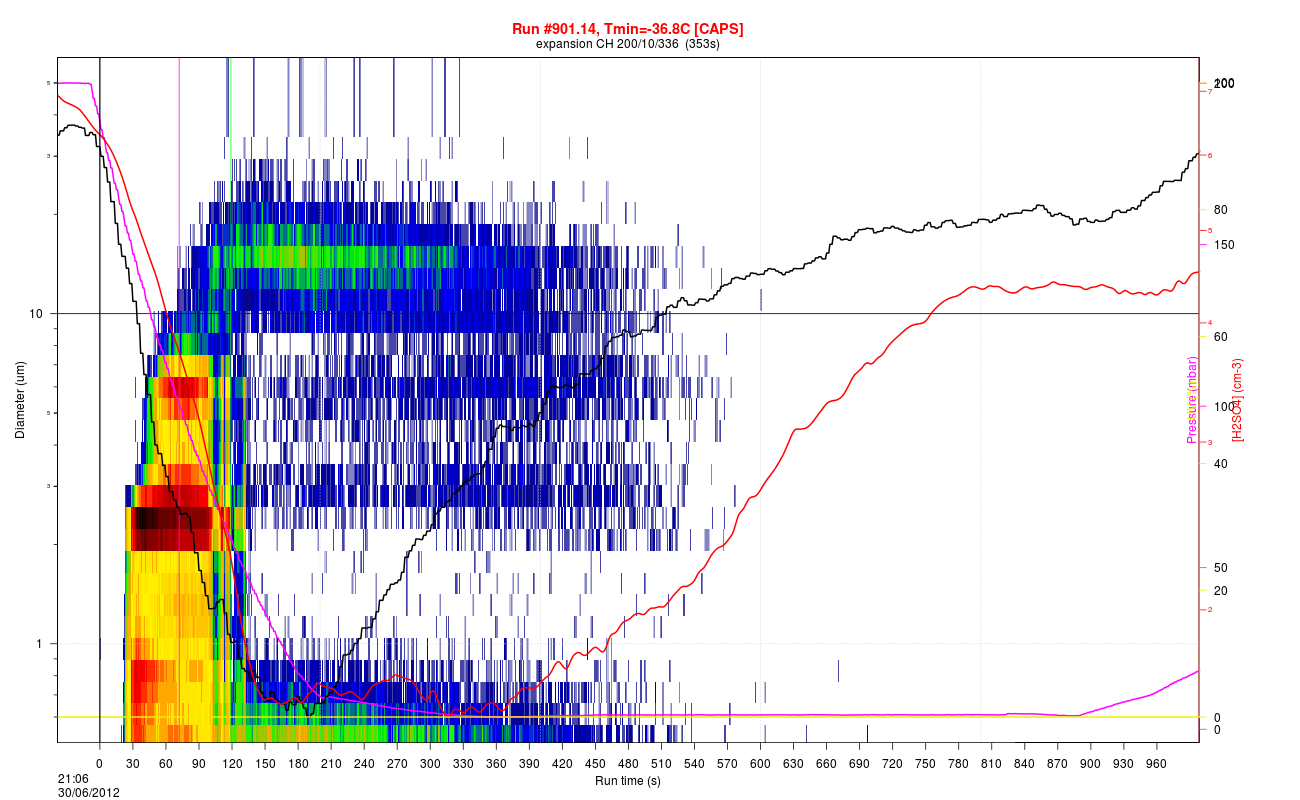
\includegraphics[scale=0.5]{runs_for_talk01.png} 
\caption{show an example picture}
\end{figure}
\end{frame}




